\let\negmedspace\undefined
\let\negthickspace\undefined
\documentclass[journal]{IEEEtran}
\usepackage[a5paper, margin=10mm, onecolumn]{geometry}
%\usepackage{lmodern} % Ensure lmodern is loaded for pdflatex
\usepackage{tfrupee} % Include tfrupee package

\setlength{\headheight}{1cm} % Set the height of the header box
\setlength{\headsep}{0mm}     % Set the distance between the header box and the top of the text

\usepackage{gvv-book}
\usepackage{gvv}
\usepackage{cite}
\usepackage{amsmath,amssymb,amsfonts,amsthm}
\usepackage{algorithmic}
\usepackage{graphicx}
\usepackage{textcomp}
\usepackage{xcolor}
\usepackage{txfonts}
\usepackage{listings}
\usepackage{enumitem}
\usepackage{mathtools}
\usepackage{gensymb}
\usepackage{comment}
\usepackage[breaklinks=true]{hyperref}
\usepackage{tkz-euclide} 
\usepackage{listings}
\def\inputGnumericTable{}                                 
\usepackage[latin1]{inputenc}                                
\usepackage{color}                                            
\usepackage{array}                                            
\usepackage{longtable}                                       
\usepackage{calc}                                             
\usepackage{multirow}                                         
\usepackage{hhline}                                           
\usepackage{ifthen}                                           
\usepackage{lscape}
\begin{document}

\bibliographystyle{IEEEtran}


\title{6.4.12}
\author{AI25BTECH11012 - GARIGE UNNATHI}
% \maketitle
% \newpage
% \bigskip
{\let\newpage\relax\maketitle}


\renewcommand{\thefigure}{\theenumi}
\renewcommand{\thetable}{\theenumi}
\setlength{\intextsep}{10pt} % Space between text and floats


\numberwithin{equation}{enumi}
\numberwithin{figure}{enumi}

\vspace{-1cm}

\textbf{Question}:\\
Find the shortest distance between the lines
\begin{align*}
 \vec{r} = \hat{i}+2\hat{j}+\hat{k} +\lambda(\hat{i}-\hat{j}+\hat{k})
\end{align*}
\begin{align*}
    \vec{r} =  2\hat{i}-1\hat{j}-1\hat{k} +\mu(2\hat{i}-\hat{j}+2\hat{k})
\end{align*}


\textbf{Solution: }

The given lines can be written in vector form as
\begin{align}
    \vec{x_1} = \myvec{1 \\2 \\1} + \lambda\myvec{1 \\-1 \\1}\\
    \vec{x_2} = \myvec{2 \\-1 \\-1} + \mu\myvec{2 \\ -1\\ 2}\\
    \vec{M} = \myvec{1 & 2 \\ -1 & -1\\1 & 2} \\
    \vec{B}-\vec{A} = \myvec{1 \\ -3 \\-2}
\end{align}

\begin{align}
    \myvec{\vec{M} & \vec{B-A}} = \myvec{1 & 2 & 1 \\ -1 & -1 & -3\\1 & 2 & -2}\\
    R_3 = R_3 + R_2\\
    = \myvec{1 & 2 & 1 \\ -1 & -1 & -3\\0 & 1 & -5}
    \end{align}
\begin{align}
    R_2 = R_2 + R_1\\
       = \myvec{1 & 2 & 1 \\ 0 & 1 & -3\\0 & 1 & -5}\\
    R_3 = R_3  - R_2 \\
         = \myvec{1 & 2 & 1 \\ 0 & 1 & -3\\0 & 0 & -2}
\end{align}

The rank of the matrix is 3 . So the given lines are skew 
\begin{align}
    \myvec{1 & -1 & 1 \\ 2 & -1 & 2}\myvec{1 & 2 \\ -1 & -1\\1 & 2}\kappa = \myvec{1 & -1 & 1 \\ 2 & -1 & 2}\myvec{1 \\ -3 \\-2} \\
  \myvec{3 & 5\\5 & 9}\kappa = \myvec{2 \\ 1}
\end{align}

The argumented matrix of the above matrix is 
\begin{align}
 \myvec{3 & 5 & 2\\5 & 9 & 1} \\
 R_2 = R_2 - \frac{5}{3}R_1 \\
 \myvec{3 & 5 & 2\\0 & \frac{2}{3} & -\frac{7}{3}} \\
R_1 = R_1 - \frac{15}{2}R_2\\
 \myvec{3 & 0 & \frac{39}{2}\\0 & \frac{2}{3} & -\frac{7}{3}}
 \end{align}
 yeilding 
\begin{align}
    \myvec{\lambda \\ -\mu} = \myvec{\frac{13}{2} \\ -\frac{7}{2}}
\end{align}
\begin{align}
    \vec{x_1} =\frac{1}{2} \myvec{15 \\ -9 \\ 15} ,
        \vec{x_2} =\frac{1}{2} \myvec{18 \\ -9 \\ 12}
\end{align}
The minimum distance between the lines is given by
\begin{align}
    \lVert \vec{x_2} - \vec{x_1} \rVert = \lVert \frac{1}{2}\myvec{3 \\ 0 \\ -3} \rVert \\
     = \frac{3\sqrt{2}}{2}
\end{align}
\begin{figure}[h!]
   \centering
   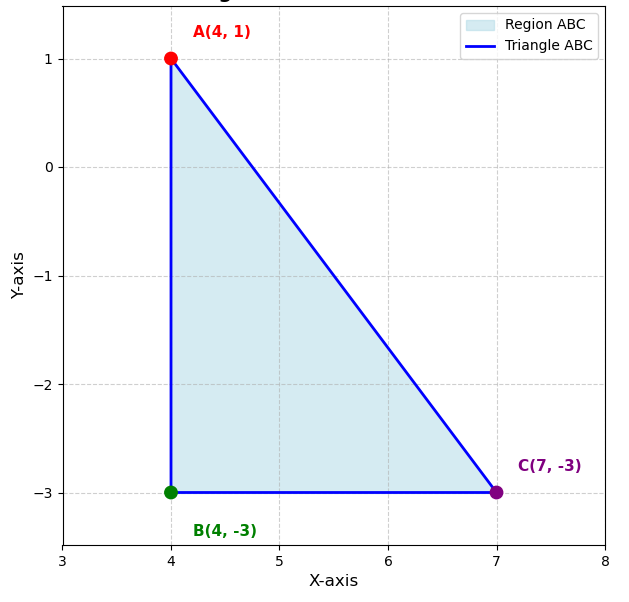
\includegraphics[width=0.7\linewidth]{/Users/unnathi/Documents/ee1030-2025/ai25btech11012/matgeo/6.4.12/figs/fig.png}
   \caption{}
   \label{stemplot}
\end{figure}


\end{document}

